\documentclass{standalone}
\usepackage[dvipsnames,svgnames,x11names]{xcolor}
\usepackage{tikz}
\usepackage{../thesismath}
\begin{document}
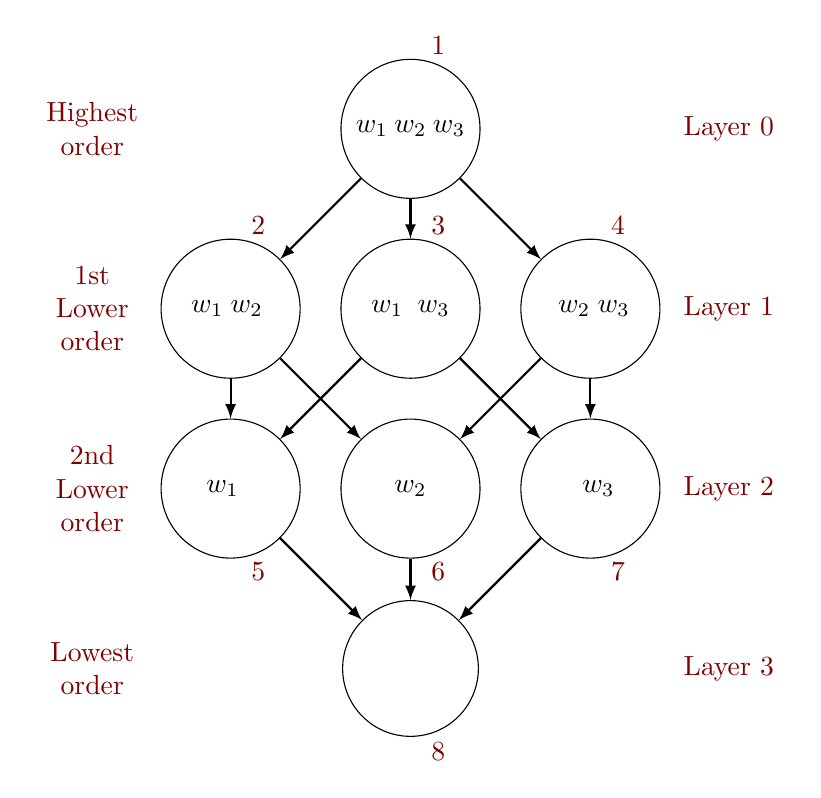
\begin{tikzpicture}
  \tikzset{
    state/.style  = {draw, circle, align = center, text centered, text width = 4.2em},
    invis/.style  = {text width = 4.2em},
    order/.style  = {align = center, text centered, text width = 4em, text = Maroon},
    number/.style = {xshift = 1em, text = Maroon},
  }

  \begin{scope}[node distance = 6.5em]
    \node [state] (000)                  {$w_1 \: w_2 \: w_3$};
    \node [invis] (000l) [left  of=000]  {};
    \node [invis] (000r) [right of=000]  {};

    \node [state] (001)  [below of=000l] {$w_1 \: w_2 \: \Skp$};
    \node [state] (010)  [below of=000]  {$w_1 \: \Skp \: w_3$};
    \node [state] (100)  [below of=000r] {$\Skp \: w_2 \: w_3$};

    \node [state] (011)  [below of=001] {$w_1 \: \Skp \: \Skp$};
    \node [state] (101)  [below of=010] {$\Skp \: w_2 \: \Skp$};
    \node [state] (110)  [below of=100] {$\Skp \: \Skp \: w_3$};

    \node [state] (111)  [below of=101] {$\Skp \: \Skp \: \Skp$};
    \node [invis] (111l) [below of=011] {};
    \node [invis] (111r) [below of=110] {};
  \end{scope}

  \begin{scope}[node distance = 5em]
    \node [order] [left of=000l]  {Highest order};
    \node [order] [left of=001]   {1st Lower order};
    \node [order] [left of=011]   {2nd Lower order};
    \node [order] [left of=111l]  {Lowest order};

    \node [order] [right of=000r] {Layer 0};
    \node [order] [right of=100]  {Layer 1};
    \node [order] [right of=110]  {Layer 2};
    \node [order] [right of=111r] {Layer 3};
  \end{scope}

  \begin{scope}[node distance = 3em]
    \node [number] [above of=000] {1};
    \node [number] [above of=001] {2};
    \node [number] [above of=010] {3};
    \node [number] [above of=100] {4};
    \node [number] [below of=011] {5};
    \node [number] [below of=101] {6};
    \node [number] [below of=110] {7};
    \node [number] [below of=111] {8};
  \end{scope}

  \path[->, >=latex, thick]
    (000) edge (001)
    (000) edge (010)
    (000) edge (100)

    (001) edge (011)
    (001) edge (101)
    (010) edge (011)
    (010) edge (110)
    (100) edge (101)
    (100) edge (110)

    (011) edge (111)
    (101) edge (111)
    (110) edge (111);
\end{tikzpicture}
\end{document}
